\documentclass[../psets.tex]{subfiles}

\pagestyle{main}
\renewcommand{\leftmark}{Problem Set \thesection}
\stepcounter{section}

\begin{document}




\section{The First and Second Laws of Thermodynamics}
\begin{enumerate}
    \item \marginnote{2/8:}Consider the following experiment with an ideal gas, and derive the relation between $\gamma$, $h$, and $h'$.\par
    Let the system sit at $P_0,T_0$ where $h=0$. Pump a little gas in (add $\Delta n$) and wait so that $T$ is back to $T_0$; measure $h$. Open the valve to air quickly to $P_0$ and close again. Justify why this can be considered a reversible adiabatic expansion. Wait so that $T$ is back to $T_0$; measure $h'$.
    \begin{center}
        \begin{tikzpicture}
            \footnotesize
            \draw [thick]
                (0,-1) circle (5.2mm)
                (-1.3,0) circle (3.2mm)
            ;
            \draw [thick,double=white,double distance=1mm]
                (2,1) -- (2,-1) to[out=-90,in=-90,looseness=2] (1.7,-1) -- (1.7,-0.3) to[out=90,in=0] (1.4,0) -- (0.06,0)
                (0,0.06) -- (0,0.5)
                (0,-0.06) -- (0,-0.5)
                (-0.06,0) -- (-0.5,0)
            ;
            \draw [thick,double=white,double distance=0.5mm] (-0.5,0) -- (-1,0);
            \draw [semithick]
                (-0.5,-0.2) -- (-0.5,0.2) (-0.6,0.2) -- (-0.4,0.2)
                (-0.2,0.5) -- (0.2,0.5) (0.2,0.4) -- (0.2,0.6)
            ;
            \draw [line width=1mm,gax] (2,-0.1) -- (2,-1) to[out=-90,in=-90,looseness=2] (1.7,-1) -- (1.7,-0.5);
    
            \draw [<->] (2.3,-0.5) -- node[right]{$h$} (2.3,-0.1);
        \end{tikzpicture}
    \end{center}
    \begin{proof}[Answer]
        % We have an isothermal constant-volume process to start. Then we have an adiabatic constant-pressure process. Then a constant-volume heating process?

        % \begin{equation*}
        %     \gamma = \frac{C_P(T)}{C_V(T)} = \frac{(\pdv*{H}{T})_P}{(\pdv*{U}{T})_V} = \pdv{H}{U} = \pdv{U}(U+PV) = 1+\dv{U}(nRT) = 1+nR\pdv{T}{U}
        % \end{equation*}

        State 1 is $P_0V_0=nRT_0$, state 2 is $(P_0+h)V_0=(n+\Delta n_1)RT_0$, and state 3 is $(P_0+h')V_0=(n+\Delta n_1+\Delta n_2)RT_0$. It follows that

        \begin{align*}
            (P_0+h)V_0 &= (n+\Delta n_1)RT_0\\
            P_0V_0+hV_0 &= nRT_0+\Delta n_1RT_0\\
            hV_0 &= \Delta n_1RT_0\\
            hV_0 &= \Delta n_1\cdot\frac{P_0V_0}{n}\\
            \frac{h}{P_0} &= \frac{\Delta n_1}{n}
        \end{align*}

        % \begin{equation*}
        %     \frac{h'-h}{P_0+h} = \frac{\Delta n_2}{n+\Delta n_1}
        % \end{equation*}

        \begin{align*}
            (P_0+h')V_0 &= (n+\Delta n_1-\Delta n_2)RT_0\\
            P_0V_0+h'V_0 &= nRT_0+\Delta n_1RT_0-\Delta n_2RT_0\\
            h'V_0 &= \Delta n_1RT_0-\Delta n_2RT_0\\
            h'V_0 &= \frac{nh}{P_0}\cdot RT_0-\Delta n_2RT_0\\
            h'V_0 &= \frac{nh}{P_0}\cdot\frac{P_0V_0}{n}-\Delta n_2\cdot\frac{P_0V_0}{n}\\
            h' &= h-\frac{P_0\Delta n_2}{n}\\
            \frac{\Delta n_2}{n} &= \frac{h-h'}{P_0} = \frac{C_P}{C_V}\frac{h}{P_0}
            % \frac{P_0}{n}(\Delta n_1+\Delta n_2) &= h+\frac{P_0\Delta n_2}{n}\\
            % \frac{P_0\Delta n_1}{n} &= h
        \end{align*}

        % \begin{equation*}
        %     (P_0+h)V_0^\gamma = 
        % \end{equation*}

        % $h'-h$ is the change in pressure from state 2 to state 3.
        \begin{align*}
            h-h' &= \frac{hC_P}{C_V}\\
            C_V(h-h') &= hC_P\\
            h(C_V-C_P) &= h'C_V\\
            \frac{h'}{h} &= \frac{C_V-C_P}{C_V}\\
            &= 1-\gamma
        \end{align*}

        % Molar internal energy is always the same; actual internal energy varies only with $n$ over the course of the experiment.

        % We WTS:
        % \begin{equation*}
        %     \frac{h'}{h} = \frac{\gamma-1}{\gamma}
        %     = 1-\frac{C_V(T)}{C_P(T)}
        %     = \frac{C_P(T)-C_V(T)}{C_P(T)}
        % \end{equation*}

        % Use $P_1V_1^\gamma=P_2V_2^\gamma$ for the adiabatic process. Volume increases during the adiabatic process. Assume the volume is volume and number of moles increase at the same rate (Charles' Law). Just consider the molecules that remain in the container to be the system during the adiabatic process. You need to introduce the adiabatic process into the math to introduce $\gamma$ into the math.
    \end{proof}
    \item 
    \begin{enumerate}
        \item $n$ moles of an ideal gas with a given $\gamma$ undergo an adiabatic expansion from $V_a$ to $V_b$. Calculate the work done and the total energy change.
        \begin{proof}[Answer]
            Let the initial pressure of the gas be $P_a$. Then
            \begin{align*}
                w &= -\int_{V_a}^{V_b}P\dd{V}\\
                &= -\int_{V_a}^{V_b}\frac{P_aV_a^\gamma}{V^\gamma}\dd{V}\\
                \Aboxed{w &= \frac{P_aV_a^\gamma}{\gamma-1}(V_b^{1-\gamma}-V_a^{1-\gamma})}
            \end{align*}
            Additionally, since the process is adiabatic (i.e., $\var{q}=0$), we know that $\Delta U=w$. Thus,
            \begin{equation*}
                \boxed{\Delta U = \frac{P_aV_a^\gamma}{\gamma-1}(V_b^{1-\gamma}-V_a^{1-\gamma})}
            \end{equation*}
        \end{proof}
        \item $n$ moles of an ideal gas with a given $\gamma$ undergo an isobaric expansion from $V_a$ to $V_b$. Calculate the work done and the total energy change.
        \begin{proof}[Answer]
            Let the constant pressure throughout the expansion be $P$. Then
            \begin{equation*}
                \boxed{w = P(V_b-V_a)}
            \end{equation*}
            Additionally, since $PV_a=nRT_a$ and $PV_b=nRT_b$, we have that
            \begin{align*}
                \Delta U &= \int_{T_a}^{T_b}C_V\dd{T}\\
                &= C_V(T_b-T_a)\\
                \Aboxed{\Delta U &= \frac{C_VP}{nR}(V_b-V_a)}
            \end{align*}
        \end{proof}
    \end{enumerate}
    \item 
    \begin{enumerate}
        \item Consider a Carnot cycle for an ideal gas. Derive the relation $Q_1/T_1+Q_2/T_2=0$ where $Q_1,Q_2$ are the heat transferred to the system along the isotherms at $T_1,T_2$.
        \begin{proof}[Answer]
            % Thing entropy, and entropy around a closed loop.
            
            The Carnot cycle is a four step process. The four steps are isothermal expansion (at $T_1$; we let $Q_1$ be the heat absorbed during this process), adiabatic expansion (the amount $Q$ of heat absorbed or released is zero), isothermal compression ($Q_2$ at $T_2$), and adiabatic compression ($Q=0$). During each of these reversible processes, there is a change in entropy $\dd{S}=\var{q_\text{rev}}/T$. Thus, the total change in entropy $\Delta S$ is given by
            \begin{align*}
                \Delta S &= \int_{T_1}^{T_1}\frac{Q_1}{T_1}\dd{T}+\int_{T_1}^{T_2}\frac{0}{T}\dd{T}+\int_{T_2}^{T_2}\frac{Q_2}{T_2}\dd{T}+\int_{T_2}^{T_1}\frac{0}{T}\dd{T}\\
                &= \frac{Q_1}{T_1}+\frac{Q_2}{T_2}
            \end{align*}
            But since $\Delta S=0$ around a closed loop (such as the Carnot cycle), we have that
            \begin{equation*}
                \frac{Q_1}{T_1}+\frac{Q_2}{T_2} = 0
            \end{equation*}
            as desired.
        \end{proof}
        \item Consider an ideal gas going from $V_1,T_1$ to $V_2,T_2$. Calculate the entropy change in terms of $V_1,V_2,T_2,T_2$.
        \begin{proof}[Answer]
            We will calculate the entropy change along two separate paths (reversible processes) that together move an ideal gas from $V_1,T_1$ to $V_2,T_2$. In particular, we go from $V_1,T_1$ to $V_2,T_1$ isothermally and then from $V_2,T_1$ to $V_2,T_2$ isochorically. If we call these processes $A$ and $B$, it follows that
            \begin{align*}
                \Delta S &= \Delta S_A+\Delta S_B\\
                &= nR\ln\frac{V_2}{V_1}+\int_{T_1}^{T_2}\frac{C_V}{T}\dd{T}\\
                \Aboxed{\Delta S &= nR\ln\frac{V_2}{V_1}+C_V\ln\frac{T_2}{T_1}}
            \end{align*}
        \end{proof}
    \end{enumerate}
    \item Practicing with partial derivatives.\par
    By expressing the internal energy state function $U$ in terms of $V$ and $T$ variables and alternatively with $P$ and $T$ variables, show that
    \begin{align*}
        \left( \pdv{U}{P} \right)_T &= \left( \pdv{U}{V} \right)_T\left( \pdv{V}{P} \right)_T&
        \left( \pdv{U}{T} \right)_P &= \left( \pdv{U}{T} \right)_V+\left( \pdv{V}{T} \right)_P\left( \pdv{U}{V} \right)_T
    \end{align*}
    Then derive that
    \begin{equation*}
        C_P-C_V = \left[ P+\left( \pdv{U}{V} \right)_T \right]\left( \pdv{V}{T} \right)_P
    \end{equation*}
    Show that
    \begin{equation*}
        \left( \pdv{U}{V} \right)_T = 0
    \end{equation*}
    for an ideal gas. And then show that
    \begin{equation*}
        C_P-C_V = nR
    \end{equation*}
    \begin{proof}[Answer]
        % We have that
        % \begin{align*}
        %     \dd{U} &= \var{q}+\var{w}\\
        %     &= T\dd{S}-P\dd{V}\\
        %     \pdv{U}{P} &= T\pdv{S}{P}-P\pdv{V}{P}
        % \end{align*}

        % \begin{align*}
        %     \pdv{U}{T} &= 
        % \end{align*}

        % \begin{align*}
        %     C_P-C_V &= \left( \pdv{V}{T} \right)_P\left( \pdv{U}{V} \right)_T
        % \end{align*}


        The total differential for $U(P,T)$ is
        \begin{equation*}
            \dd{U} = \left( \pdv{U}{P} \right)_T\dd{P}+\left( \pdv{U}{T} \right)_P\dd{T}
        \end{equation*}
        It contains the two partial derivatives for which we want to find expressions. Thus, we need only manipulate an analogous equation into the above form. To do so, we use the total differential for $U(V,T)$
        \begin{equation*}
            \dd{U} = \left( \pdv{U}{V} \right)_T\dd{V}+\left( \pdv{U}{T} \right)_V\dd{T}
        \end{equation*}
        This is close, but we need $\dd{P}$, not $\dd{V}$. Thus, we substitute the total differential for $V(P,T)$
        \begin{equation*}
            \dd{V} = \left( \pdv{V}{P} \right)_T\dd{P}+\left( \pdv{V}{T} \right)_P\dd{T}
        \end{equation*}
        into the above expression to get
        \begin{align*}
            \dd{U} &= \left( \pdv{U}{V} \right)_T\left[ \left( \pdv{V}{P} \right)_T\dd{P}+\left( \pdv{V}{T} \right)_P\dd{T} \right]+\left( \pdv{U}{T} \right)_V\dd{T}\\
            &= \left( \pdv{U}{V} \right)_T\left( \pdv{V}{P} \right)_T\dd{P}+\left( \pdv{U}{V} \right)_T\left( \pdv{V}{T} \right)_P\dd{T}+\left( \pdv{U}{T} \right)_V\dd{T}\\
            &= \left( \pdv{U}{V} \right)_T\left( \pdv{V}{P} \right)_T\dd{P}+\left[ \left( \pdv{U}{V} \right)_T\left( \pdv{V}{T} \right)_P+\left( \pdv{U}{T} \right)_V \right]\dd{T}
        \end{align*}
        The first two equations follow by comparing the above with the total differential for $U(P,T)$.\par
        % \begin{align*}
        %     \dd{H} &= \dd{(U+PV)}\\
        %     &= \dd{U}+P\dd{V}+V\dd{P}\\
        %     &= \var{q}+V\dd{P}\\
        %     &= T\dd{S}+V\dd{P}
        % \end{align*}
        % \begin{align*}
        %     U &= H-PV\\
        %     \dd{U} &= \dd{H}-P\dd{V}-V\dd{P}\\
        %     \pdv{U}{T} &= \pdv{H}{T}-P\pdv{V}{T}-V\pdv{P}{T}\\
        %     \left( \pdv{U}{T} \right)_V+\left( \pdv{V}{T} \right)_P\left( \pdv{U}{V} \right)_T &= \pdv{H}{T}-P\pdv{V}{T}-V\pdv{P}{T}\\
        %     \pdv{H}{T}-\left( \pdv{U}{T} \right)_V &= \left( \pdv{V}{T} \right)_P\left( \pdv{U}{V} \right)_T+P\pdv{V}{T}+V\pdv{P}{T}
        % \end{align*}
        % It follows that
        % \begin{align*}
        %     C_P-C_V &= \left( \pdv{H}{T} \right)_P-\left( \pdv{U}{T} \right)_V\\
        %     &= P\pdv{V}{T}+V\pdv{P}{T}\\
        %     &= \left[ P+\left( \pdv{U}{V} \right)_T \right]\left( \pdv{V}{T} \right)_P
        % \end{align*}

        % \begin{equation*}
        %     \left( \pdv{U}{V} \right)_T = P+\left( \pdv{U}{V} \right)_T
        % \end{equation*}


        It follows from the second equation and the definition of enthalpy that
        \begin{align*}
            \left( \pdv{T}(H-PV) \right)_P &= \left( \pdv{U}{V} \right)_T\left( \pdv{V}{T} \right)_P+\left( \pdv{U}{T} \right)_V\\
            \left( \pdv{H}{T} \right)_P-P\left( \pdv{V}{T} \right)_P-V\left( \pdv{P}{T} \right)_P &= \left( \pdv{U}{V} \right)_T\left( \pdv{V}{T} \right)_P+\left( \pdv{U}{T} \right)_V
        \end{align*}
        Noting that $\pdv*{P}{T}=0$ for $P$ a constant function (the derivative is taken at constant pressure) and employing the definitions of $C_P,C_V$ gives us
        \begin{align*}
            C_P-P\left( \pdv{V}{T} \right)_P-V\cdot 0 &= \left( \pdv{U}{V} \right)_T\left( \pdv{V}{T} \right)_P+C_V\\
            C_P-C_V &= \left( \pdv{U}{V} \right)_T\left( \pdv{V}{T} \right)_P+P\left( \pdv{V}{T} \right)_P\\
            &= \left[ P+\left( \pdv{U}{V} \right)_T \right]\left( \pdv{V}{T} \right)_P
        \end{align*}
        as desired.\par
        Since the internal energy $U$ of an ideal gas is solely a function of temperature $T$, taking the partial derivative of $U$ with respect to $V$ is equivalent to taking the derivative of a constant function, and thus we clearly have
        \begin{equation*}
            \left( \pdv{U}{V} \right)_T = 0
        \end{equation*}\par
        It follows since $V=nRT/P$ by the ideal gas law that
        \begin{align*}
            C_P-C_V &= \left[ P+\left( \pdv{U}{V} \right)_T \right]\left( \pdv{V}{T} \right)_P\\
            &= \left[ P+0 \right]\frac{nR}{P}\\
            &= nR
        \end{align*}
        as desired.
    \end{proof}
    \item Write that $\dd{U}=T\dd{S}-P\dd{V}$ and derive the following two relations.
    \begin{align*}
        \left( \pdv{S}{T} \right)_V &= \frac{C_V}{T}&
        \left( \pdv{S}{V} \right)_T &= \frac{1}{T}\left[ P+\left( \pdv{U}{V} \right)_T \right]
    \end{align*}
    \begin{proof}[Answer]
        The total differential of $U(T,V)$ is
        \begin{equation*}
            \dd{U} = \left( \pdv{U}{T} \right)_V\dd{T}+\left( \pdv{U}{V} \right)_T\dd{V}
        \end{equation*}
        Thus, we have that
        \begin{align*}
            T\dd{S}-P\dd{V} &= \left( \pdv{U}{T} \right)_V\dd{T}+\left( \pdv{U}{V} \right)_T\dd{V}\\
            \dd{S} &= \frac{1}{T}\left( \pdv{U}{T} \right)_V\dd{T}+\frac{1}{T}\left[ P+\left( \pdv{U}{V} \right)_T \right]\dd{V}\\
            &= \frac{C_V}{T}\dd{T}+\frac{1}{T}\left[ P+\left( \pdv{U}{V} \right)_T \right]\dd{V}
        \end{align*}
        The two equations follow by comparing the above with the total differential for $S(T,V)$, given by
        \begin{equation*}
            \dd{S} = \left( \pdv{S}{T} \right)_V\dd{T}+\left( \pdv{S}{V} \right)_T\dd{V}
        \end{equation*}
    \end{proof}
    \item Problem 21-10. Show your work.\par
    It has been found experimentally that $\Delta_\text{vap}\overline{S}\approx\SI{88}{\joule\per\kelvin\per\mole}$ for many nonassociated liquids. This rough rule of thumb is called \textbf{Trouton's rule}. Use the following data to test the validity of Trouton's rule.
    \begin{center}
        \small
        \renewcommand{\arraystretch}{1.2}
        \begin{tabular}{
            l
            c
            S[table-format=3.2]
            S[table-format=2.2]
            S[table-format=2.2]
        }
            \toprule
            Substance & {$t_\text{fus}/\si{\celsius}$} & {$t_\text{vap}/\si{\celsius}$} & {$\Delta_\text{fus}\overline{H}/\si{\kilo\joule\per\mole}$} & {$\Delta_\text{vap}\overline{H}/\si{\kilo\joule\per\mole}$}\\
            \midrule
            Pentane            & -129.7 & 36.06 & 8.42  & 25.79\\
            Hexane             & -95.3  & 68.73 & 13.08 & 28.85\\
            Heptane            & -90.6  & 98.5  & 14.16 & 31.77\\
            Ethylene oxide     & -111.7 & 10.6  & 5.17  & 25.52\\
            Benzene            & 5.53   & 80.09 & 9.95  & 30.72\\
            Diethyl ether      & -116.3 & 34.5  & 7.27  & 26.52\\
            Tetrachloromethane & -23    & 76.8  & 3.28  & 29.82\\
            Mercury            & -38.83 & 356.7 & 2.29  & 59.11\\
            Bromine            & -7.2   & 58.8  & 10.57 & 29.96\\
            \bottomrule
        \end{tabular}
    \end{center}
    \begin{proof}[Answer]
        We know that
        \begin{equation*}
            \Delta_\text{vap}\overline{S} = \frac{\Delta_\text{vap}\overline{H}}{t_\text{vap}}
        \end{equation*}
        Thus, for pentane (for example), we have that
        \begin{equation*}
            \Delta_\text{vap}\overline{S}(\text{pentane}) = \frac{\SI{25.79}{\kilo\joule\per\mole}}{\SI{36.06}{\celsius}}
            = \frac{\SI{2.579e4}{\joule\per\mole}}{\SI{309.21}{\kelvin}}
            = \SI{83.41}{\joule\per\kelvin\per\mole}
        \end{equation*}
        We can run the same calculation for all of the other values to learn that
        \begin{align*}
            \Delta_\text{vap}\overline{S}(\text{hexane}) &= \SI{84.39}{\joule\per\kelvin\per\mole}\\
            \Delta_\text{vap}\overline{S}(\text{heptane}) &= \SI{85.47}{\joule\per\kelvin\per\mole}\\
            \Delta_\text{vap}\overline{S}(\text{ethylene oxide}) &= \SI{89.92}{\joule\per\kelvin\per\mole}\\
            \Delta_\text{vap}\overline{S}(\text{benzene}) &= \SI{86.97}{\joule\per\kelvin\per\mole}\\
            \Delta_\text{vap}\overline{S}(\text{diethyl ether}) &= \SI{86.19}{\joule\per\kelvin\per\mole}\\
            \Delta_\text{vap}\overline{S}(\text{tetrachloromethane}) &= \SI{85.20}{\joule\per\kelvin\per\mole}\\
            \Delta_\text{vap}\overline{S}(\text{mercury}) &= \SI{93.84}{\joule\per\kelvin\per\mole}\\
            \Delta_\text{vap}\overline{S}(\text{bromine}) &= \SI{90.24}{\joule\per\kelvin\per\mole}
        \end{align*}
        Since the mean of this set of values of $\Delta_\text{vap}\overline{S}$ is $87.29\approx 88$ and the standard deviation is relatively small, the given data supports Trouton's rule.
    \end{proof}
    \item Problem 21-37. Show your reasoning.\par
    Given that $\tilde{\nu}_1=\SI{1321.3}{\per\centi\meter}$, $\tilde{\nu}_2=\SI{750.8}{\per\centi\meter}$, $\tilde{\nu}_3=\SI{1620.3}{\per\centi\meter}$, $\tilde{A}_0=\SI{7.9971}{\per\centi\meter}$, $\tilde{B}_0=\SI{0.4339}{\per\centi\meter}$, and $\tilde{C}_0=\SI{0.4103}{\per\centi\meter}$, calculate the standard molar entropy of \ce{NO2_{(g)}} at \SI{298.15}{\kelvin}. (Note that \ce{NO2_{(g)}} is a bent triatomic molecule.) How does your value compare with that in Table 21.2?
    \begin{proof}[Answer]
        Given molecular data, it will be easiest to calculate the standard molar entropy by means of the partition function $Q$. We can do this with the help of the equation
        \begin{equation*}
            S = k_B\ln Q+k_BT\left( \pdv{\ln Q}{T} \right)_{N,V}
        \end{equation*}
        To see if we can employ the $Q=q^N/N!$ approximation, we apply the following condition, where $P=\SI{1}{\bar}$, $T=\SI{298.15}{\kelvin}$, $m=\SI[per-mode=symbol]{46.01}{\gram\per\mole}=\SI{7.640e-26}{\kilo\gram}$, and the rest of the terms are fundamental constants.
        \begin{align*}
            \frac{N}{V}\left( \frac{h^2}{8mk_BT} \right)^{3/2} &\stackrel{?}{\ll} 1\\
            \frac{P}{RT}\left( \frac{h^2}{8mk_BT} \right)^{3/2} &\stackrel{?}{\ll} 1\\
            \num{5.596e-8} &\stackrel{\checkmark}{\ll} 1
        \end{align*}
        Indeed we can, so thus we write
        \begin{align*}
            S &= k_B\ln\frac{q^N}{N!}+k_BT\left( \pdv{\ln q^N/N!}{T} \right)_V\\
            &= Nk_B\ln q-k_B\ln N!+k_BTN\left( \pdv{\ln q}{T} \right)_V-k_BTN\left( \pdv{\ln N!}{T} \right)_V\\
            &= Nk_B\ln q-Nk_B\ln N+Nk_B+Nk_BT\left( \pdv{\ln q}{T} \right)_V\\
            &= Nk_B+Nk_B\ln\frac{q}{N}+Nk_BT\left( \pdv{\ln q}{T} \right)_V
        \end{align*}
        Now for a nonlinear polyatomic molecule,
        \begin{equation*}
            q(V,T) = \left( \frac{2\pi Mk_BT}{h^2} \right)^{3/2}V\cdot\frac{\sqrt{\pi}}{\sigma}\sqrt{\frac{T^3}{\Theta_{\text{rot},A}\Theta_{\text{rot},B}\Theta_{\text{rot},C}}}\cdot\prod_{j=1}^{3n-6}\frac{\e[-\Theta_{\text{vib},j}/2T]}{1-\e[-\Theta_{\text{vib},j}/T]}\cdot g_{e1}\e[D_e/k_BT]
        \end{equation*}
        It follows that for \ce{NO2} in particular,
        \begin{equation*}
            q(V,T) = \left( \frac{2\pi Mk_BT}{h^2} \right)^{3/2}V\cdot\frac{\sqrt{\pi}}{2}\sqrt{\frac{T^3}{\Theta_{\text{rot},A}\Theta_{\text{rot},B}\Theta_{\text{rot},C}}}\cdot\prod_{j=1}^{3}\frac{\e[-\Theta_{\text{vib},j}/2T]}{1-\e[-\Theta_{\text{vib},j}/T]}\cdot\e[D_e/k_BT]
        \end{equation*}
        Then since
        \begin{align*}
            \ln q &= \ln\left[ \left( \frac{2\pi Mk_BT}{h^2} \right)^{3/2}V\cdot\frac{\sqrt{\pi}}{2}\sqrt{\frac{T^3}{\Theta_{\text{rot},A}\Theta_{\text{rot},B}\Theta_{\text{rot},C}}}\cdot\prod_{j=1}^{3}\frac{\e[-\Theta_{\text{vib},j}/2T]}{1-\e[-\Theta_{\text{vib},j}/T]}\cdot\e[D_e/k_BT] \right]\\
            &= \ln\left[ \left( \frac{2\pi Mk_BT}{h^2} \right)^{3/2}V \right]+\frac{1}{2}\ln\frac{T^3\pi}{4\Theta_{\text{rot},A}\Theta_{\text{rot},B}\Theta_{\text{rot},C}}+\sum_{j=1}^3\ln\left[ \frac{\e[-\Theta_{\text{vib},j}/2T]}{1-\e[-\Theta_{\text{vib},j}/T]} \right]+\frac{D_e}{k_BT}\\
            &= \frac{3}{2}\ln T+\frac{1}{2}\cdot 3\ln T+\sum_{j=1}^3\left[ -\frac{\Theta_{\text{vib},j}}{2T}-\ln\left( 1-\e[-\Theta_{\text{vib},j}/T] \right) \right]+\frac{D_e}{k_BT}+\text{terms not involving }T\\
            &= 3\ln T+\sum_{j=1}^3\left[ -\frac{\Theta_{\text{vib},j}}{2T}-\ln\left( 1-\e[-\Theta_{\text{vib},j}/T] \right) \right]+\frac{D_e}{k_BT}+\text{terms not involving }T
        \end{align*}
        and
        \begin{align*}
            \left( \pdv{\ln q}{T} \right)_V &= \frac{3}{T}+\sum_{j=1}^3\left[ \frac{\Theta_{\text{vib},j}}{2T^2}+\frac{(\Theta_{\text{vib},j}/T^2)\e[-\Theta_{\text{vib},j}/T]}{1-\e[-\Theta_{\text{vib},j}/T]} \right]-\frac{D_e}{k_BT^2}\\
            Nk_BT\left( \pdv{\ln q}{T} \right)_V &= 3Nk_B+Nk_B\sum_{j=1}^3\left[ \frac{\Theta_{\text{vib},j}}{2T}+\frac{(\Theta_{\text{vib},j}/T)\e[-\Theta_{\text{vib},j}/T]}{1-\e[-\Theta_{\text{vib},j}/T]} \right]-\frac{ND_e}{T}
        \end{align*}
        we have that
        \begin{align*}
            S ={}& Nk_B+Nk_B\ln q-Nk_B\ln N+Nk_BT\left( \pdv{\ln q}{T} \right)_V\\
            \begin{split}
                ={}& Nk_B+Nk_B\left\{ \ln\left[ \left( \frac{2\pi Mk_BT}{h^2} \right)^{3/2}V \right]+\frac{1}{2}\ln\frac{T^3\pi}{4\Theta_{\text{rot},A}\Theta_{\text{rot},B}\Theta_{\text{rot},C}}\right.\\
                & \left. +\sum_{j=1}^3\ln\left[ \frac{\e[-\Theta_{\text{vib},j}/2T]}{1-\e[-\Theta_{\text{vib},j}/T]} \right]+\frac{D_e}{k_BT} \right\}\\
                & -Nk_B\ln N+3Nk_B+Nk_B\sum_{j=1}^3\left[ \frac{\Theta_{\text{vib},j}}{2T}+\frac{(\Theta_{\text{vib},j}/T)\e[-\Theta_{\text{vib},j}/T]}{1-\e[-\Theta_{\text{vib},j}/T]} \right]-\frac{ND_e}{T}
            \end{split}\\
            \begin{split}
                ={}& 4Nk_B+Nk_B\left\{ \ln\left[ \left( \frac{2\pi Mk_BT}{h^2} \right)^{3/2}V \right]+\frac{1}{2}\ln\frac{T^3\pi}{4\Theta_{\text{rot},A}\Theta_{\text{rot},B}\Theta_{\text{rot},C}} \right.\\
                & \left. +\sum_{j=1}^3\left[ -\frac{\Theta_{\text{vib},j}}{2T}-\ln\left( 1-\e[-\Theta_{\text{vib},j}/T] \right) \right]+\frac{D_e}{k_BT} \right\}\\
                & -Nk_B\ln N+Nk_B\sum_{j=1}^3\left[ \frac{\Theta_{\text{vib},j}}{2T}+\frac{(\Theta_{\text{vib},j}/T)\e[-\Theta_{\text{vib},j}/T]}{1-\e[-\Theta_{\text{vib},j}/T]} \right]-\frac{ND_e}{T}
            \end{split}\\
            \begin{split}
                ={}& Nk_B\left\{ 4+\ln\left[ \left( \frac{2\pi Mk_BT}{h^2} \right)^{3/2}\frac{V}{N} \right]+\frac{1}{2}\ln\frac{T^3\pi}{4\Theta_{\text{rot},A}\Theta_{\text{rot},B}\Theta_{\text{rot},C}} \right.\\
                & \left. +\sum_{j=1}^3\left[ -\ln\left( 1-\e[-\Theta_{\text{vib},j}/T] \right) \right] \right.\\
                & \left. +\sum_{j=1}^3\left[ \frac{(\Theta_{\text{vib},j}/T)\e[-\Theta_{\text{vib},j}/T]}{1-\e[-\Theta_{\text{vib},j}/T]} \right] \right\}
            \end{split}\\
            \begin{split}
                \frac{\overline{S}}{R} ={}& 4+\ln\left[ \left( \frac{2\pi Mk_BT}{h^2} \right)^{3/2}\frac{RT}{PN_A} \right]+\frac{1}{2}\ln\frac{T^3\pi}{4\Theta_{\text{rot},A}\Theta_{\text{rot},B}\Theta_{\text{rot},C}}\\
                & +\sum_{j=1}^3\left[ \frac{(\Theta_{\text{vib},j}/T)\e[-\Theta_{\text{vib},j}/T]}{1-\e[-\Theta_{\text{vib},j}/T]}-\ln\left( 1-\e[-\Theta_{\text{vib},j}/T] \right) \right]
            \end{split}
        \end{align*}
        We now construct the needed values from the given data on \ce{NO2}. In particular, since $\Theta_\text{vib}=h\nu/k_B=hc\tilde{\nu}/k_B$, we have that
        \begin{align*}
            \Theta_{\text{vib},1} &= \frac{hc\tilde{\nu}_1}{k_B}&
                \Theta_{\text{vib},2} &= \frac{hc\tilde{\nu}_2}{k_B}&
                    \Theta_{\text{vib},3} &= \frac{hc\tilde{\nu}_3}{k_B}\\
            &= \SI{1901}{\kelvin}&
                &= \SI{1080}{\kelvin}&
                    &= \SI{2331}{\kelvin}
        \end{align*}
        Additionally, since $\Theta_\text{rot}=\hbar^2/2Ik_B$ and $\tilde{X}_0=h/8\pi^2cI$, we have that
        \begin{equation*}
            \Theta_\text{rot} = \frac{h^2}{8\pi^2Ik_B}
            = \frac{hc}{k_B}\cdot\frac{h}{8\pi^2cI}
            = \frac{hc\tilde{X}_0}{k_B}
        \end{equation*}
        Thus,
        \begin{align*}
            \Theta_{\text{rot},A} &= \frac{hc\tilde{A}_0}{k_B}&
                \Theta_{\text{rot},B} &= \frac{hc\tilde{B}_0}{k_B}&
                    \Theta_{\text{rot},C} &= \frac{hc\tilde{C}_0}{k_B}\\
            &= \SI{11.50}{\kelvin}&
                &= \SI{0.6241}{\kelvin}&
                    &= \SI{0.5902}{\kelvin}
        \end{align*}
        The value of $M$ was given above (as $m$ in the molecular partition function criterion), and everything else is a fundamental constant. The one exception is pressure, which we take to be standard (i.e., $\SI{1}{\bar}=\SI{1e5}{\pascal}$). Choosing values such that all units cancel gives us
        \begin{equation*}
            \boxed{\overline{S} = \SI{234.3}{\joule\per\mole\per\kelvin}}
        \end{equation*}
    \end{proof}
    \item Problem 19-55.\par
    Use the rigid rotator-harmonic oscillator model and the data in Table 18.2 to plot $\overline{C}_P(T)$ for \ce{CO_{(g)}} from \SI{300}{\kelvin} to \SI{1000}{\kelvin}. Compare your result with the expression given in Problem 19-43.
    \begin{proof}[Answer]
        For a linear molecule,
        \begin{equation*}
            \frac{C_V}{Nk_B} = \frac{5}{2}+\sum_{j=1}^{3n-5}\left( \frac{\Theta_{\text{vib},j}}{T} \right)^2\frac{\e[-\Theta_{\text{vib},j}/T]}{(1-\e[-\Theta_{\text{vib},j}/T])^2}
        \end{equation*}
        In particular, for a linear diatomic molecule,
        \begin{equation*}
            \frac{C_V}{Nk_B} = \frac{5}{2}+\left( \frac{\Theta_\text{vib}}{T} \right)^2\frac{\e[-\Theta_\text{vib}/T]}{(1-\e[-\Theta_\text{vib}/T])^2}
        \end{equation*}
        Thus, since $C_P-C_V=Nk_B$, we have that
        \begin{align*}
            C_P &= \frac{7}{2}Nk_B+Nk_B\left( \frac{\Theta_\text{vib}}{T} \right)^2\frac{\e[-\Theta_\text{vib}/T]}{(1-\e[-\Theta_\text{vib}/T])^2}\\
            \overline{C}_V(T) &= \frac{7}{2}R+R\left( \frac{\Theta_\text{vib}}{T} \right)^2\frac{\e[-\Theta_\text{vib}/T]}{(1-\e[-\Theta_\text{vib}/T])^2}
        \end{align*}
        where $\Theta_\text{vib}=\SI{3103}{\kelvin}$ by Table 18.2. This function is plotted below in red, and the expression given in Problem 19-43 is plotted below in blue. They clearly follow the same general trend but nevertheless display not insignificant differences in their trajectory.
        \begin{figure}[H]
            \centering
            \includegraphics[width=0.3\linewidth]{../../ExtFiles/pset2-8.png}
            \begin{tikzpicture}[remember picture,overlay]
                \small
                \node [below=7mm] at (-2.595,0) {T/K};
                \node [rotate=90,above=7mm] at (-5.07,1.6) {$\overline{C}_P/R$};
                \footnotesize
                % \draw (-5.07,0) rectangle ++(4.95,3.2);
                \draw [stealth-stealth] (-5.07,3.5) -- ++(0,-3.5) node[below right,yshift=-1mm]{300} node[above left,xshift=-1mm]{3.4} -- ++(5.3,0);
                \foreach \x in {-4.245,-3.42,...,-0.12} {
                    \draw (\x,0.1) -- ++(0,-0.2);
                }
                \foreach \y in {0.8,1.6,...,4} {
                    \draw (-4.97,\y) -- ++(-0.2,0);
                }
                \node [below] at (-0.12,-0.1) {1000};
                \node [left] at (-5.17,3.2) {4.2};
            \end{tikzpicture}
        \end{figure}
    \end{proof}
\end{enumerate}




\end{document}